\chapter{Capitolo 4: Algoritmi basati sulla distanza}
In questo capitolo vengono illustrati i principali algoritmi utilizzati per la costruzione degli alberi evolutivi. L'obiettivo è quello di trovare una soluzione al cosiddetto \textit{problema degli alberi basati sulla distanza}, ma prima è necessario introdurre alcuni concetti, tra cui la matrice delle distanze.

\section{Matrice delle distanze}
Dati due punti, $x$ e $y$, la \textit{distanza} può essere vista come loro "lontananza" in uno spazio $k$-dimensionale. Nella fattispecie è una funzione $d(x,y)$ che possiede le seguenti proprietà \cite{molaCagliari}:
\begin{enumerate}
	\item \textit{non negatività}:
	\[d(x,y)\geq 0\hspace{2em} \forall \: x,y\in R^k\]
	\item \textit{identità}:
	\[d(x,y)=0 \; \leftrightarrow \; x=y\]
	\item \textit{simmetria}:
	\[d(x,y)=d(y,x)\hspace{2em} \forall \: x,y\in R^k\]
	\item \textit{disuguaglianza triangolare}:
	\[d(x,y)\leq d(x,z)+d(y,z)\hspace{2em} \forall \: x,y,z\in R^k\]
\end{enumerate}
Date $n$ unità, calcolando la distanza per ogni coppia di elementi\footnote{Ci sono vari modi per calcolare la distanza tra due elementi, ad esempio attraverso la distanza Euclidea, quella di Manhattan, di Minkowski e così via.} si ottiene una \textit{matrice delle distanze $n \times n$}, definita nel seguente modo \cite{ingrassiaStatistica}:
\[
D = \begin{pmatrix}
0 & d_{12} & d_{13} & \ldots & d_{1n} \\ 
d_{21} & 0 & d_{23} & \ldots & d_{2n} \\ 
d_{31} & d_{32} & 0 & \ldots & d_{3n} \\ 
\vdots & \vdots & \vdots & \ddots & \vdots \\ 
d_{n1} & d_{n2} & \ldots & \ldots & 0
\end{pmatrix}
\hspace{3em}dove\;d(x_i,x_j)=D_i,_j
\]
Poiché è costruita a partire dalle distanze, ne eredita le proprietà precedentemente elencate.
\newline
Ciascun valore $D_i,_j$ può assumere significati diversi in base al contesto, ad esempio può indicare il numero di simboli diversi tra i geni $i$ e $j$ nell'allineamento di sequenze di DNA\footnote{L'allineamento è il processo attraverso il quale si misura la similarità tra due o più sequenze.}, come mostrato nell'esempio sottostante:
\begin{figure}[h!]
	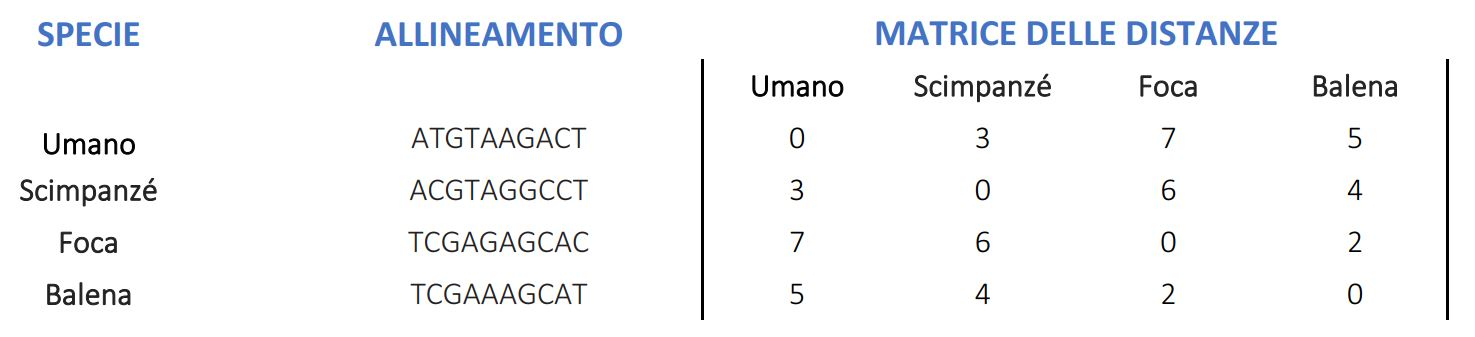
\includegraphics[width=\linewidth]{distance_matrix_example.jpg}
 	\caption{Esempio di matrice delle distanze.}
  	\label{fig:DistanceMatrix}
\end{figure}
\newline
Nella figura 5 è possibile notare che la sequenza di DNA della foca risulta molto più simile a quella della balena, in quanto la distanza è $2$, rispetto all'umano, con cui la distanza è $7$.
\newpage

\section{Problema degli alberi basati sulla distanza}
Gli algoritmi basati sulla distanza utilizzano la matrice delle distanze per costruire gli alberi evolutivi, dove le foglie corrispondono alle entità biologiche presenti nella matrice, mentre i nodi interni rappresentano gli antenati non noti. Per poter conoscere quale è la distanza tra due foglie, e quindi conoscere quanto sono legate tra loro, è necessario associare un valore non negativo (peso) a ciascun arco, pertanto la lunghezza del cammino in tale albero è la somma dei suoi pesi. Si definisce, quindi, la \textit{distanza evolutiva} tra due entità biologiche corrispondenti alle foglie $i$ e $j$ di un albero $T$ come la lunghezza dell'unico cammino che li collega, ed è indicato come $d_i,_j(T)$ \cite{bioinfalganactivelearningapproachparttwo}. In altre parole è dato dalla somma dei pesi degli archi che ci sono tra $i$ e $j$.
\newline
Si dice che un albero $T$ si \textit{adatta} ad una matrice delle distanze $D$ se per ogni coppia di foglie $i$ e $j$ si ha che $D_i,_j=d_i,_j(T)$, ovvero l'elemento nella riga $i$ e colonna $j$ è uguale alla lunghezza del cammino che le collega (distanza evolutiva), in tal caso sia la matrice che l'albero vengono definiti \textit{additivi}. Qualora invece non esista un albero che si adatti alla matrice, allora è \textit{non additiva} \cite{UniCaliforniaadditivetree}.
\newline
Si riporta di seguito un esempio che mostra un albero che si adatta alla matrice delle distanze mostrata nella sezione precedente.
\begin{figure}[h!]
	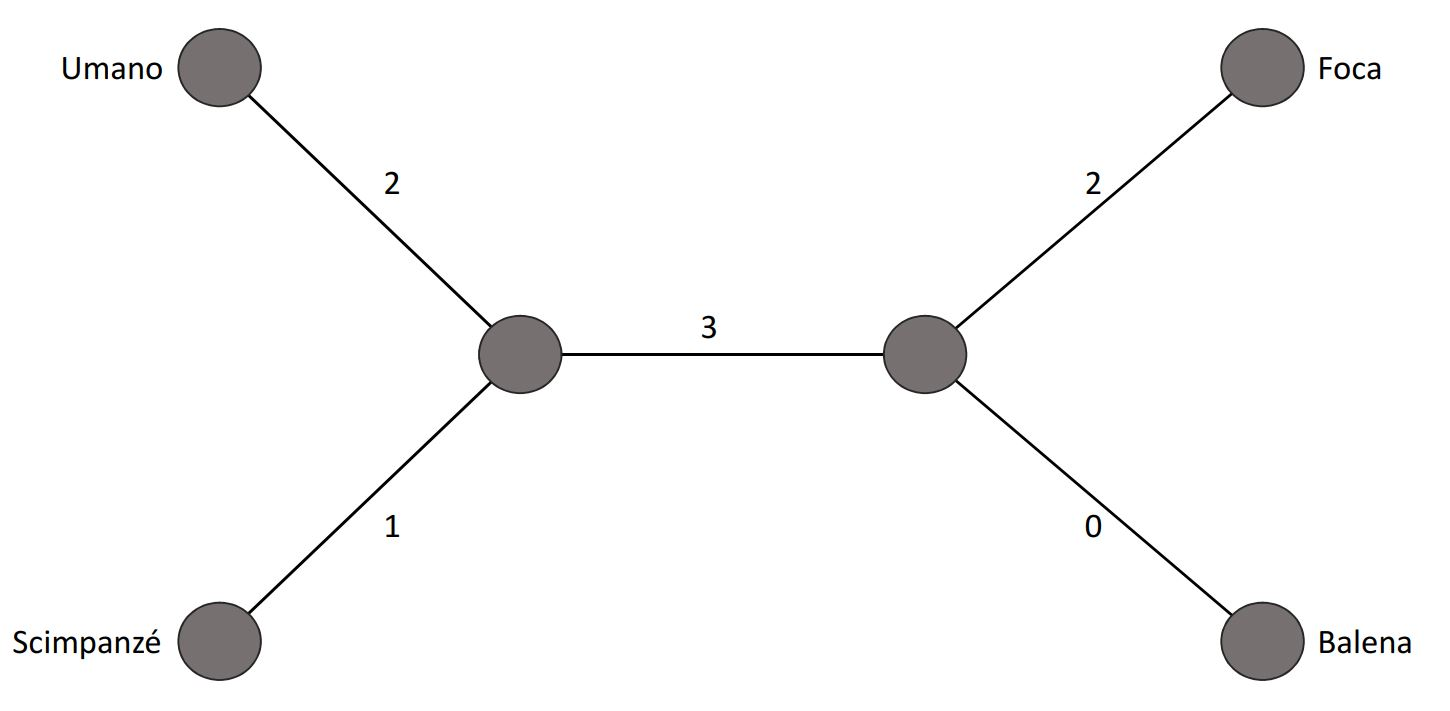
\includegraphics[width=\linewidth]{unrooted_tree_created_by_figure_5.jpg}
 	\caption{Albero evolutivo senza radice costruito a partire dalla matrice \textbf{additiva} della figura 5.}
  	\label{fig:EvolutionaryTreeExample}
\end{figure}
\newline
Ci possono essere più alberi che si adattano ad una matrice, quindi come si può scegliere l'albero giusto? Si nota che quello in figura 6 ha tutti i vertici di grado diverso da due e viene definito \textit{albero semplice}. 
\newpage
Una loro caratteristica importante è che per ogni matrice delle distanze additiva esiste un unico albero semplice che si adatta alla matrice stessa.
\newline
Adesso è possibile dare una definizione al problema accennato all'inizio del capitolo:
\begin{center}
\textbf{Problema degli alberi basati sulla distanza:}
\newline
\textit{Dato in \textbf{input} una matrice delle distanze additiva si ottiene in \textbf{output} un albero evolutivo semplice.}
\end{center}

\section{Algoritmo per il problema degli alberi basati sulla distanza}
L'obiettivo è quello di costruire un albero semplice $T$ che si adatti alla matrice delle distanze additiva $D$.
\newline
Si prenda in considerazione la matrice della figura 5, riportata di seguito\footnote{Per brevità si definisce u=umano, s=scimpanzé, f=foca, b=balena.}:
\[
D = \bordermatrix{\text{specie}&u&s&f&b\cr
                u& 0 & 3 & 7 & 5\cr
                s& 3 & 0 & 6 & 4\cr
                f& 7 & 6 & 0 & 2\cr
                b& 5 & 4 & 2 & 0}
\]
\newline
L'idea di base dell'algoritmo è che all'elemento più piccolo della matrice corrisponda a delle foglie \textit{vicine} nel rispettivo albero, ovvero che abbiano lo stesso genitore, con $D_i,_j=d_i,_j(T)$.
\newline
Poiché l'elemento più piccolo della matrice è $D_{fb}$, il cui valore è $2$, si può supporre che $f$ e $b$ siano vicini. Si indica con $p$ il genitore non noto delle due foglie. La situazione è mostrata di seguito.
\begin{figure}[h!]
\centering
	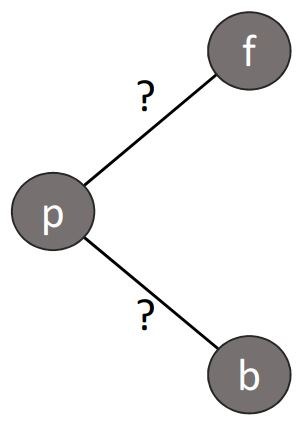
\includegraphics[height=3cm, width=2cm]{distance_between_f_b.jpg}
 	\caption{Foglie vicine con un generico genitore $p$.}
  	\label{fig:neighborsleaves}
\end{figure}
\newline
Come si può calcolare la distanza tra $f$ e $p$ ($d_{fp}$) e tra $b$ e $p$ ($d_{bp}$)? Le uniche informazioni a disposizione sono le distanze tra le quattro foglie presenti nella matrice e che $f$, $p$ sono vicini. Il passo successivo dell'algoritmo è mostrato di seguito.
\begin{figure}[h!]
\centering
	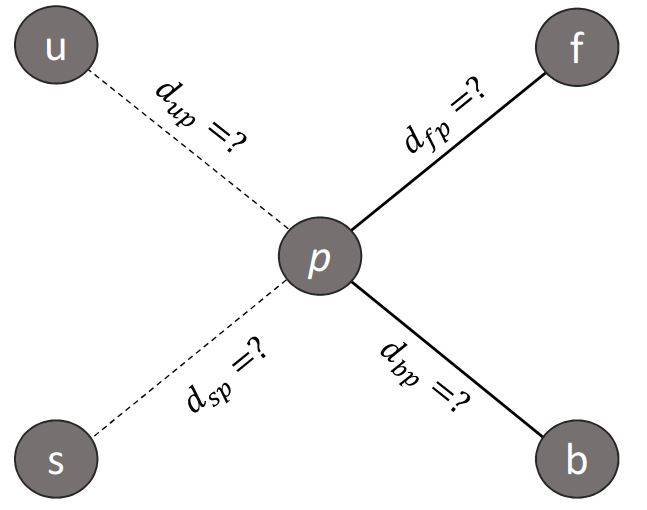
\includegraphics[height=9cm, width=7cm, keepaspectratio]{distance_between_f_b_part_2.jpg}
 	\caption{Le quattro foglie $u$, $s$, $f$ e $d$.}
  	\label{fig:neighborsleaves_2}
\end{figure}
\newline
Nella figura 8 sono state aggiunte le foglie $u$ ed $s$, ma il loro arco è tratteggiato in quanto ancora non è possibile sapere come sono collocate nell'albero.
\newline
In questo step viene scelta casualmente una foglia tra $u$ ed $s$ e viene sfruttato il valore della sua distanza rispetto a $p$ per poter calcolare $d_{fp}$ e $d_{bp}$ (in questo caso si sceglie $u$). Per far ciò è quindi necessario scrivere le distanze tra le foglie nel seguente modo:
\[d_{fu}=d_{fp}+d_{up}\]
\[d_{fb}=d_{fp}+d_{bp}\]
\[d_{bu}=d_{bp}+d_{up}\]
\[d_{up}=\frac{d_{fu}+d_{bu}-d_{fb}}2=
\frac{(d_{fp}+d_{up})+(d_{bp}+d_{up})-(d_{fp}+d_{bp})}2=\]
\[=\frac{d_{fp}+d_{up}+d_{bp}+d_{up}-d_{fp}-d_{bp}}2=
\frac{d_{up}+d_{up}}2=
\frac{2d_{up}}2=d_{up}
\]
Perché scrivere $d_{up}$ in quel modo? Perché non si conosce il peso dei nodi interni ma solo quello delle foglie grazie alla matrice di partenza, di conseguenza poiché è additiva, $d_{fu}=D_{fu}$, $d_{fb}=D_{fb}$ e $d_{bu}=D_{bu}$. Quindi si può scrivere $d_{up}$ nel seguente modo:
\[d_{up}=\frac{d_{fu}+d_{bu}-d_{fb}}2=\frac{D_{fu}+D_{bu}-D_{fb}}2\]
A questo punto si è in grado di calcolare la distanza tra $f$ e $p$ e tra $b$ e $p$, ricavandola dalle uguaglianze trovate poc'anzi. Per prima cosa si calcola $d_{fp}$:
\[d_{fu}=d_{fp}+d_{up} \rightarrow d_{fp}=d_{fu}-d_{up}=D_{fu}-D_{up}=\]
\[=D_{fu}-\frac{D_{fu}+D_{bu}-D_{fb}}2=\frac{2D_{fu}-D_{fu}-D_{bu}+D_{fb}}2=\]
\[=\frac{D_{fu}+D_{fb}-D_{bu}}2=\frac{7+2-5}2=2\]
Quindi $d_{fp}=2$. In modo analogo si calcola $d_{bp}$:
\[d_{bu}=d_{bp}+d_{up} \rightarrow d_{bp}=d_{bu}-d_{up}=D_{bu}-D_{up}=\]
\[=D_{bu}-\frac{D_{fu}+D_{bu}-D_{fb}}2=\frac{2D_{bu}-D_{fu}-D_{bu}+D_{fb}}2=\]
\[\frac{D_{bu}+D_{fb}-D_{fu}}2=\frac{5+2-7}2=0\]
Quindi $d_{bp}=0$. Il risultato di questo passo dell'algoritmo è il seguente albero:
\begin{figure}[h!]
\centering
	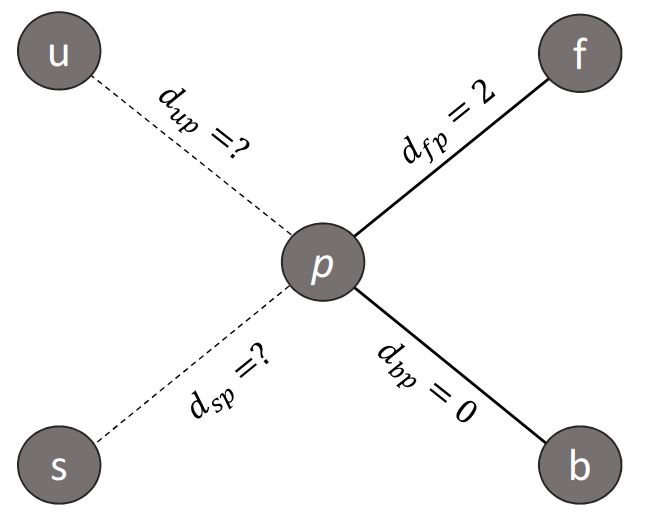
\includegraphics[height=9cm, width=7cm, keepaspectratio]{distance_between_f_b_part_3.jpg}
 	\caption{Albero con le distanze $d_{fp}$ e $d_{bp}$.}
  	\label{fig:neighborsleaves_3}
\end{figure}
\newline
Il prossimo step consiste nel trovare la distanza tra $u$ e $p$ e tra $s$ e $p$: dalla matrice D sappiamo che $D_{fu}=d_{fu}=7$ e dai calcoli precedenti che $d_{fp}=2$, quindi $d_{up}=d_{fu}-d_{fp}=7-2=5$. Stesso ragionamento anche per $d_{sp}$, ovvero $d_{sp}=d_{bs}-d_{bp}=4-0=4$.
\newline
L'albero corrispondente è:
\newpage
\begin{figure}[h!]
\centering
	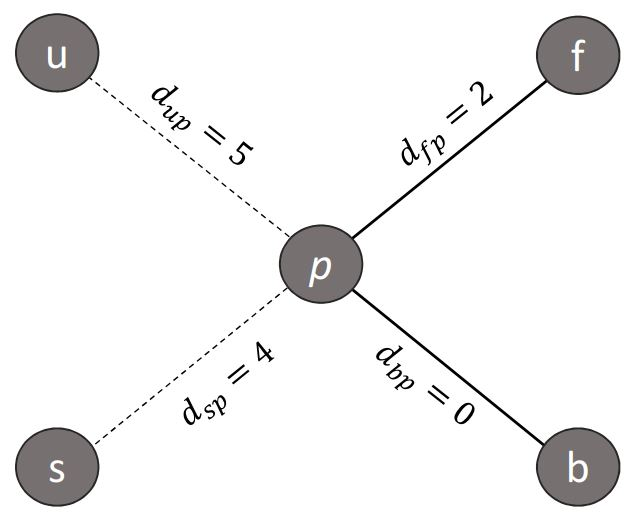
\includegraphics[height=9cm, width=7cm, keepaspectratio]{distance_between_f_b_part_4.jpg}
 	\caption{Albero con le distanze $d_{fp}$, $d_{bp}$, $d_{up}$ e $d_{sp}$.}
  	\label{fig:neighborsleaves_3}
\end{figure}
Adesso è necessario fare due modifiche alla matrice D, la prima consiste nel mettere una riga e colonna in più, definite $p$, che rappresentano le distanze appena trovate, ottenendo quindi la seguente matrice:
\[
D = \bordermatrix{\text{specie}&u&s&f&b&p\cr
                u& 0 & 3 & 7 & 5 & 5\cr
                s& 3 & 0 & 6 & 4 & 4\cr
                f& 7 & 6 & 0 & 2 & 2\cr
                b& 5 & 4 & 2 & 0 & 0\cr
                p&  5 & 4 & 2 & 0 & 0}
\]
la seconda invece consiste nel togliere le righe e colonne appartenenti a $f$ e $b$, in quanto i rispettivi nodi sono già aggiunti all'albero, pertanto non più utili. Quindi:
\[
D = \bordermatrix{\text{specie}&u&s&p\cr
                u& 0 & 3 & 5\cr
                s& 3 & 0 & 4\cr
                p&  5 & 4 & 0}
\]
Anche se adesso si conoscono le distanze di tutte le foglie con il genitore $p$, rimane comunque da capire se $u$ e $s$ abbiano altri genitori. Si ricorda, infatti, che i loro archi sono stati tratteggiati in quanto ancora non si conosce la loro collocazione nell'albero.
Per risolvere questo problema basta applicare ricorsivamente i passi precedenti, quindi si individua l'elemento più piccolo della matrice ($d_{su}$) e si suppone che $s$ e $u$ siano vicini e quindi che abbiano un genitore non noto $k$, come mostrato in figura 11.
\newpage
\begin{figure}[h!]
\centering
	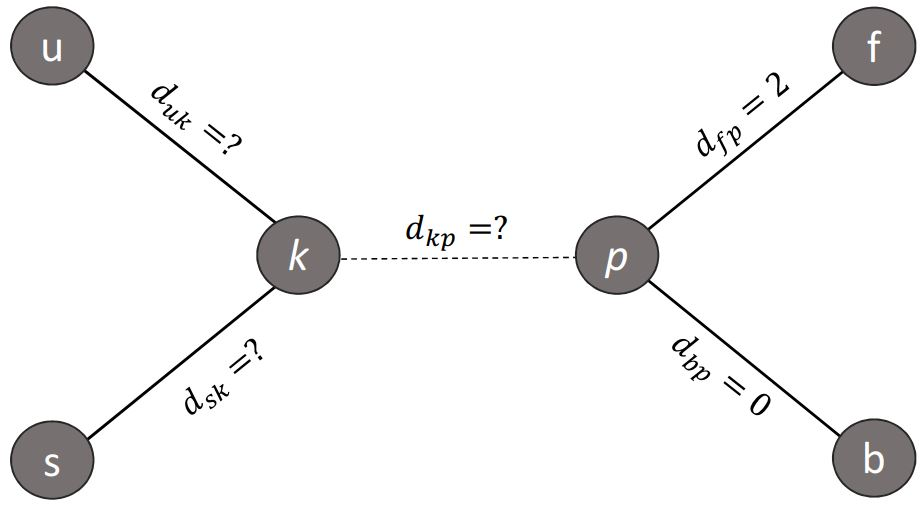
\includegraphics[height=13cm, width=11cm, keepaspectratio]{distance_between_s_u.jpg}
 	\caption{Albero con il nuovo genitore non noto $k$.}
  	\label{fig:neighborsleaves_3}
\end{figure}
Viene scelto il nodo $p$ e sfruttato il valore della sua distanza rispetto ad $u$ e $s$ per poter calcolare $d_{uk}$ e $d_{sk}$. Adattando le formule di pagina $31$ con i dati attuali, si ottiene:
\[d_{pk}=\frac{d_{up}+d_{sp}-d_{us}}2=
\frac{(d_{uk}+d_{pk})+(d_{sk}+d_{pk})-(d_{uk}+d_{sk})}2=\]
\[=\frac{2d_{pk}}2=d_{pk}
\]
Adesso si può calcolare $d_{uk}$:
\[d_{up}=d_{uk}+d_{pk} \rightarrow d_{uk}=D_{up}-D_{pk}=D_{up}-\frac{D_{up}+D_{sp}-D_{us}}2=\]
\[=\frac{D_{up}+D_{us}-D_{sp}}2=2\]

%-\frac{(D_{uk}+D_{pk})+(D_{sk}+D_{pk})-(D_{uk}+D_{sk})}2=\]
%\[=\frac{(D_{up}+D_{us}-D_{sp})}2=2
%\]
E $d_{sk}$:
\[d_{sp}=d_{sk}+d_{pk} \rightarrow d_{sk}=D_{sp}-D_{pk}=D_{sp}-\frac{D_{up}+D_{sp}-D_{us}}2=\]
\[=\frac{D_{sp}+D_{us}-D_{up}}2=1\]
Applicando le distanze trovate all'albero della figura 11, si ottiene:
\newpage
\begin{figure}[h!]
\centering
	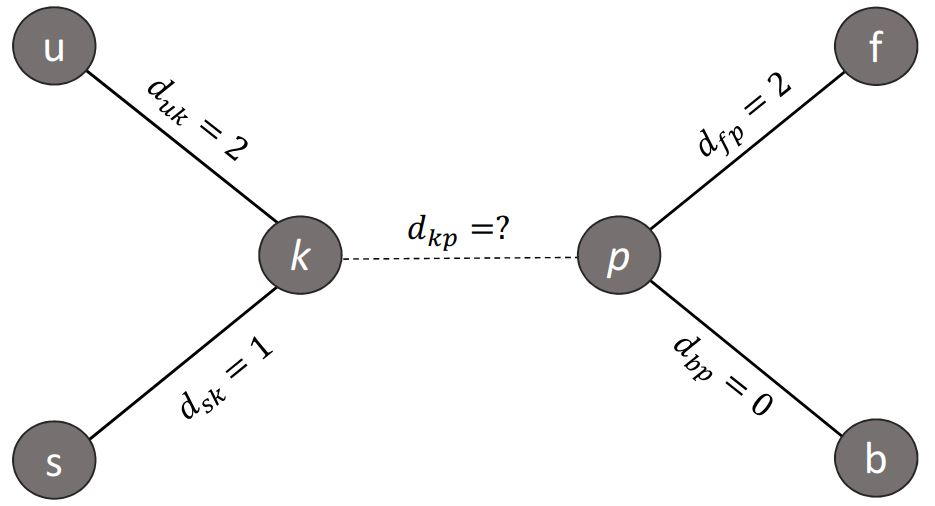
\includegraphics[height=13cm, width=11cm, keepaspectratio]{distance_between_s_u_part_2.jpg}
 	\caption{Albero con le distanze $d_{uk}$ e $d_{sk}$ calcolate.}
  	\label{fig:neighborsleaves_3}
\end{figure}
Dopo aver trovato ricorsivamente la distanza delle foglie dai propri genitori e di conseguenza aver aggiornato la matrice, rimane un ultimo passo da completare, ovvero calcolare la distanza tra $k$ e $p$: in precedenza si era calcolata la distanza tra $u$ e $p$ e tra $s$ e $p$, quindi basta sottrarre tali valori a quelli trovati adesso e troviamo $d_{kp}$.
\[d_{kp}=d_{sp}-d_{sk}=4-1=d_{up}-d_{uk}=5-2=3\]
L'albero finale che si ottiene è il seguente:
\begin{figure}[h!]
\centering
	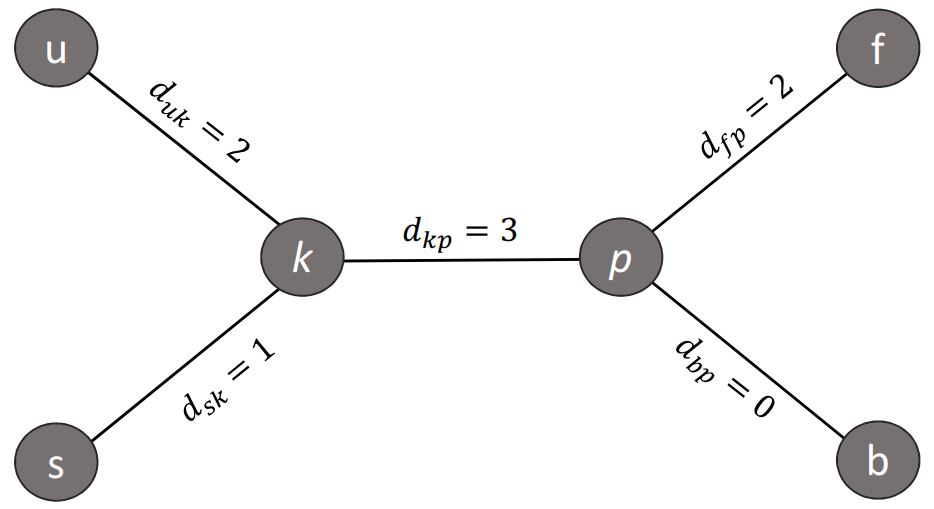
\includegraphics[height=13cm, width=11cm, keepaspectratio]{distance_between_s_u_part_4.jpg}
 	\caption{Albero evolutivo semplice con tutte le distanze calcolate.}
  	\label{fig:neighborsleaves_4}
\end{figure}
\newline
L'algoritmo è terminato. Tuttavia vi è una criticità che viene mostrata nella sezione successiva.

\subsection{Complessità temporale}
Per calcolare la complessità nel tempo dell'algoritmo possiamo suddividerlo in tre step, di seguito elencati.
\begin{enumerate}
	\item \textit{Step 1}: Trovare il minimo in una matrice di dimensione $n \times n$.
	\newline
	Si suppone l'utilizzo di un algoritmo di ricerca lineare, la cui complessità nel caso pessimo, dato in input un vettore di lunghezza $n$, è pari a $O(n)$. Poiché questa operazione deve essere effettuata per tutte le $n$ righe, otteniamo che:
	\[T(step 1)=O(n) \times O(n) \simeq O(n^2)\]
	\item \textit{Step 2}: Trovare il genitore per ogni coppia di foglie e calcolare la distanza di tutte le $n$ foglie  rispetto al genitore stesso.
	\newline
	Questa operazione deve essere fatta $n$ volte, quindi $O(n)$. In seguito dovrà essere aggiornata la matrice; per semplicità si suppone che il costo rimanga invariato, quindi $O(1)$.
	\[T(step 2)=O(n)+O(1) \simeq O(n)\]
	\item \textit{Step 3}: Calcolare le distanze tra i genitori trovati nello step precedente.
	\newline
	Poiché per ogni coppia di foglie esiste un genitore, allora il costo sarà:
	\[T(step 3)=O(n/2)\]
\end{enumerate}
Adesso è sufficiente sommare le tre complessità e si trova quella totale dell'algoritmo:
\[T(totale)=T(step 1)+T(step 2)+T(step 3)=\]
\[=O(n^2)+O(n)+O(n/2) \simeq O(n^2) \]

\newpage

\section{Albero Additivo}
L'algoritmo mostrato nella sezione precedente presenta una criticità, infatti riesce a risolvere il problema degli \textit{alberi basati sulla distanza} solamente se l'elemento più piccolo della matrice D corrisponde a due foglie \textit{vicine} nell'albero T. Ma questo non è necessariamente vero, infatti ci sono matrici delle distanze che, seppur additive (e quindi $ \forall i,j\in V,D_{ij}=d_{ij}(T)$), non possiedono come elemento più piccolo una coppia di foglie con lo stesso genitore. Si deve, quindi, approcciare il problema in modo diverso: invece di cercare le foglie vicine in un albero (come visto nella sezione precedente), l'idea di base dell'algoritmo è quella di costruirlo aggiungendole una alla volta. Per far ciò è necessario conoscere il peso degli archi che collegano le foglie ai rispettivi genitori. Questi prendono il nome di \textit{arti}. Tutti gli altri sono definiti \textit{archi interni} \cite{cambridgeBioInf}. Tale operazione andrà effettuata in termini di matrice delle distanze D, dato che non si conosce l'albero T fino a che l'algoritmo non è completato.
\newline
Il primo problema che si pone è quello di calcolare il peso degli arti: data una foglia $j$, si denota con \textit{limbweight(j)} il peso dell'arco che collega $j$ al suo genitore \cite{bioinfvideoAdditive}.

\begin{center}
\textbf{Teorema del peso degli arti:}
\newline
\textit{Data una matrice delle distanze additiva $D$ ed una foglia $j$, \textit{limbweight(j)} è uguale al valore minimo di $\frac{D_{j,i}+D_{j,k}-D_{i,k}}{2}$ tra le foglie $i$ e $k$\footnote{Si omette la dimostrazione, che è comunque consultabile nel libro \textit{Bioinformatics Algorithms, An Active Learning Approach, Vol II} di Compeau P., Pevzner P.} \cite{bioinfalganactivelearningapproachparttwo}} .
\end{center}

A titolo esemplificativo si riporta l'applicazione del teorema alla seguente matrice\footnote{Per brevità si definisce f=foca, b=balena, u=umano, s=scimpanzé. Inoltre si ricorda che questi rappresentano le foglie nel rispettivo albero evolutivo $T$.}:
\[
D = \bordermatrix{\text{specie}&u&s&f&b\cr
                u& 0 & 3 & 7 & 5\cr
                s& 3 & 0 & 6 & 4\cr
                f& 7 & 6 & 0 & 2\cr
                b& 5 & 4 & 2 & 0}
\]
Supponendo di non conoscere quali sono le foglie vicine, si vuole calcolare il peso dell'arto di $f$, quindi:
\[limbweight(f)=\frac{D_{f,i}+D_{f,k}-D_{i,k}}{2}\]
Al posto $i$ e $k$ si sostituiscono di volta in volta i valori delle foglie (escluso $f$), ovvero:
\begin{itemize}
	\item $i=u$ e $k=s$:
	\[limbweight_{us}(f)=\frac{D_{f,u}+D_{f,s}-D_{u,s}}{2}=\frac{7+6-3}{2}=\frac{10}{2}=5\]
	\item $i=u$ e $k=b$:
	\[limbweight_{ub}(f)=\frac{D_{f,u}+D_{f,b}-D_{u,b}}{2}=\frac{7+2-5}{2}=\frac{4}{2}=2\]
	\item $i=s$ e $k=b$:
	\[limbweight_{sb}(f)=\frac{D_{f,s}+D_{f,b}-D_{s,b}}{2}=\frac{6+2-4}{2}=\frac{4}{2}=2\]
\end{itemize}
Si può concludere dicendo che \textit{limbweight(f)}=$2$.
\newline
Tali operazioni hanno una complessità di $O(n^2)$, in quanto ogni elemento della matrice viene confrontato con tutti gli altri elementi, che sono $n-2$ (escluso $f$ e sé stesso). Questa operazione viene eseguita tante volte quante sono le foglie da analizzare, ovvero $n-2$, quindi $O(n-2)\times O(n-2)\simeq O(n^2)$.
\newline
Ora che si è in grado di calcolare il peso degli arti si può illustrare l'algoritmo che risolve la criticità spiegata ad inizio della sezione.
Sia $D$ una matrice delle distanze additiva di dimensione $n\times n$, tale che il suo elemento più piccolo non corrisponde a due foglie \textit{vicine} nel rispettivo albero $T$, ovvero:
\[
D = \bordermatrix{\text{specie}&f&b&u&s\cr
                f& 0 & 13 & 21 & 22\cr
                b& 13 & 0 & 12 & 13\cr
                u& 21 & 12 & 0 & 13\cr
                s& 22 & 13 & 13 & 0}
\]
\newpage
Quello che si dovrà ottenere è il seguente albero:
\begin{figure}[h!]
\centering
	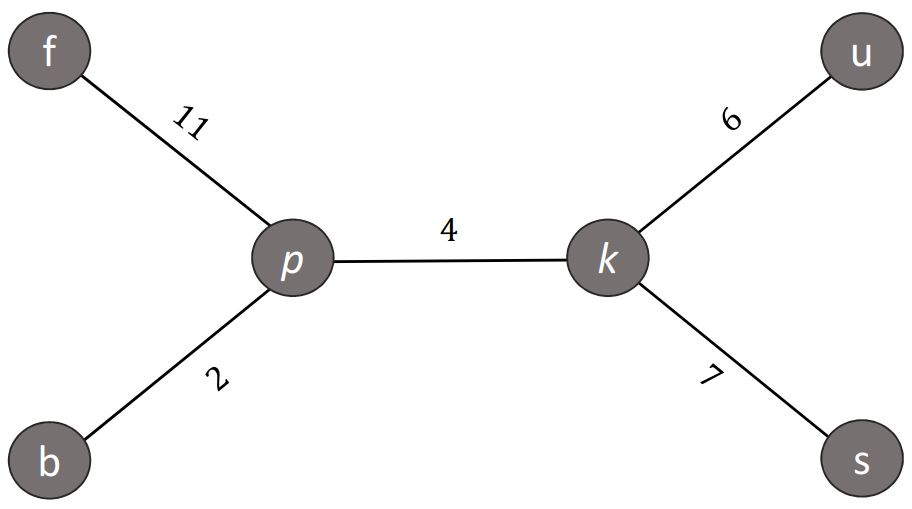
\includegraphics[height=12cm, width=10cm, keepaspectratio]{additive_tree_1.jpg}
 	\caption{Albero T ottenuto dalla matrice D.}
  	\label{fig:additivePhylogeny_1}
\end{figure}
\newline
Per prima cosa si sceglie casualmente dalla matrice una foglia $b$ e si calcola \textit{limbweight(b)}:
\[limbweight(b)=\frac{D_{b,i}+D_{b,k}-D_{i,k}}{2}\]
\begin{itemize}
	\item $i=f$ e $k=u$:
	\[limbweight_{fu}(b)=\frac{D_{b,f}+D_{b,u}-D_{f,u}}{2}=\frac{13+12-21}{2}=\frac{4}{2}=2\]
	\item $i=f$ e $k=s$:
	\[limbweight_{fs}(b)=\frac{D_{b,f}+D_{b,s}-D_{f,s}}{2}=\frac{13+13-22}{2}=\frac{4}{2}=2\]
	\item $i=u$ e $k=s$:
	\[limbweight_{us}(b)=\frac{D_{b,u}+D_{b,s}-D_{u,s}}{2}=\frac{12+13-13}{2}=\frac{12}{2}=6\]
\end{itemize}
Quindi $limbweight(b)=2$.
\newline
Poiché abbiamo calcolato il peso dell'arto di $b$ è necessario aggiornare la matrice, sottraendo $limbweight(b)$ a tutti gli elementi lungo la riga e la colonna $b$ (escluso lo zero sulla diagonale). Si ottiene una nuova matrice $D^{spoglia_{b}}$ che verrà utilizzata successivamente per costruire l'albero.
\[
D^{spoglia_{b}}= \bordermatrix{\text{specie}&f&b&u&s\cr
                f& 0 & {\color{Blue} 11} & 21 & 22\cr
                b& {\color{Blue} 11} & 0 & {\color{Blue} 10} & {\color{Blue} 11}\cr
                u& 21 & {\color{Blue} 10} & 0 & 13\cr
                s& 22 & {\color{Blue} 11} & 13 & 0}
\]
Poiché la riga e la colonna $b$ non forniscono informazioni aggiuntive, sarebbe inutile tenerle, pertanto si tolgono dalla matrice $D^{spoglia_{b}}$. Il risultato è il seguente:
\[
D^{tagliata_{b}}= \bordermatrix{\text{specie}&f&u&s\cr
                f& 0 & 21 & 22\cr
                u& 21 & 0 & 13\cr
                s& 22 & 13 & 0}
\]
Adesso si può ottenere l'albero evolutivo $T$ eseguendo ricorsivamente i seguenti step:
\begin{enumerate}
	\item Scegliere casualmente una foglia $j$, calcolare $limbweight(j)$, costruire $D^{spoglia_{j}}$ e  $D^{tagliata_{j}}$ (eliminando la riga e la colonna $j$). Ripetere queste operazioni fino a che non si ottiene una matrice $D^{tagliata}$ di dimensioni $2 \times 2$.
	\item Costruire un albero $T^{tagliato}$ a partire da $D^{tagliata}$ trovata nello step precedente. All'inizio sarà composto solamente da una coppia di foglie ed un arco che le collega.
	\item Identificare il punto di $T^{tagliato}$ in cui la foglia $j$ deve essere inserita. Questo passo verrà spiegato successivamente.
	\item Aggiungere la foglia $j$ ed aggiornare il peso degli archi nell'albero. La ripetizione di questo punto e quello precedete permette di costruirlo di volta in volta fino al suo completamento.
\end{enumerate}
Si prende la matrice $D^{tagliata_{b}}$ e si applicano i passaggi sopraelencati, quindi si sceglie la foglia $s$ e si calcola \textit{limbweight(s)}:
\[limbweight(s)=\frac{D_{s,i}+D_{s,k}-D_{i,k}}{2}\]
\begin{itemize}
	\item $i=f$ e $k=u$:
	\[limbweight(s)=\frac{D_{s,f}+D_{s,u}-D_{f,u}}{2}=\frac{13+22-21}{2}=\frac{14}{2}=7\]
\end{itemize}
Si sottrae $limbweight(s)$ a tutti gli elementi lungo la riga e la colonna $s$ presenti in $D^{tagliata_{b}}$, ottenendo così:
\[
D^{spoglia_{s}}= \bordermatrix{\text{specie}&f&u&s\cr
                f& 0 & 21 & {\color{Blue} 15}\cr
                u& 21 & 0 & {\color{Blue} 6}\cr
                s& {\color{Blue} 15} & {\color{Blue} 6} & 0}
\]
A questo punto si elimina la foglia $s$ da $D^{spoglia_{s}}$:
\[
D^{tagliata_{s}}= \bordermatrix{\text{specie}&f&u\cr
                f& 0 & 21\cr
                u& 21 & 0}
\]
Il risultato è una matrice $2 \times 2$, quindi si può cominciare a costruire l'albero:
\begin{figure}[h!]
\centering
	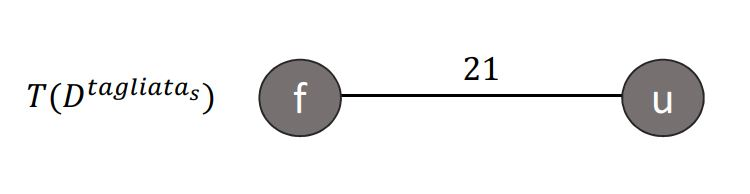
\includegraphics[height=9cm, width=7cm, keepaspectratio]{additive_tree_2.jpg}
 	\caption{Albero ottenuto dalla matrice $D^{tagliata_{s}}$.}
  	\label{fig:additivePhylogeny_2}
\end{figure}
\newline
Lo step successivo è quello di individuare il punto di $T(D^{tagliata_{s}})$ in cui $s$ deve essere inserito. Per fare ciò si consideri la matrice $D^{spoglia_{s}}$. Dal \textit{teorema del peso degli arti} si ha che:
\[limbweight(s)=\frac{D^{spoglia_{s}}_{f,s}+D^{spoglia_{s}}_{s,u}-D^{spoglia_{s}}_{f,u}}{2}\]
Ma poiché $D^{spoglia_{s}}$ è una matrice ottenuta da $D^{tagliata_{b}}$ togliendo il peso dell'arto di $s$, allora $limbweight(s)=0$. Questo significa che:
\[
0=\frac{D^{spoglia_{s}}_{f,s}+D^{spoglia_{s}}_{s,u}-D^{spoglia_{s}}_{f,u}}{2} \rightarrow D^{spoglia_{s}}_{f,u}=D^{spoglia_{s}}_{f,s}+D^{spoglia_{s}}_{s,u}
\]
Questo significa che $s$ sta tra il cammino di $f$ ed $u$ (come si può notare dalla figura 15), in particolar modo a distanza $D^{spoglia_{s}}_{s,u}$ da $s$, ovvero $6$.
\newline
Dato che il punto di attacco sta lungo l'arco\footnote{Il punto di attacco può può essere anche su un vertice già esistente, in tal caso si connette $s$ a tale vertice.}, si crea un nodo interno che rappresenta un genitore non noto $k$ e si aggiunge $s$, il cui arto ha un peso pari a $limbweight(s)=7$.
\newpage
Adesso si aggiunge la foglia e si aggiorna il peso degli altri archi, quindi:
\begin{figure}[h!]
\centering
	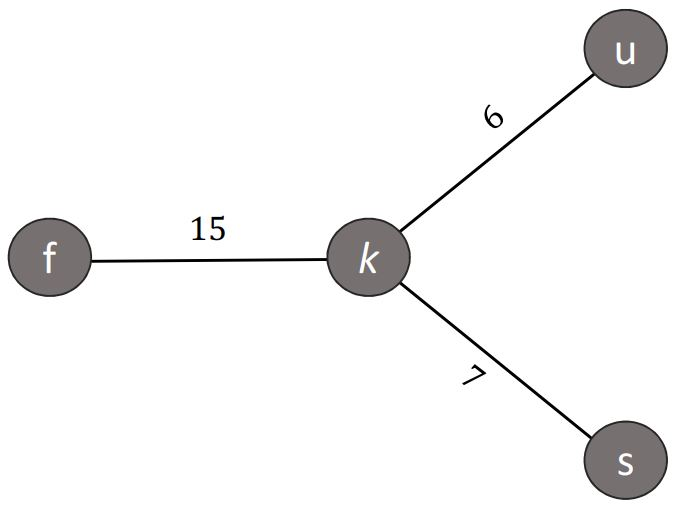
\includegraphics[height=8cm, width=6cm, keepaspectratio]{additive_tree_3.jpg}
 	\caption{Albero con la nuova foglia $s$.}
  	\label{fig:additivePhylogeny_3}
\end{figure}
\newline
$d_{sk}=7$ è il peso dell'arto di $s$ che è già stato calcolato in precedenza; $d_{uk}=D^{spoglia_{s}}_{s,u}=6$ è ottenuto sottraendo $limbweight(s)=7$ a \newline $D^{tagliata_{b}}_{s,u}=13$; $d_{fk}=15$ è dato da $D^{spoglia_{s}}_{f,u}-d_{uk}=21-6=15$.
\newline
Infine si ripetono gli ultimi step dell'algoritmo fino a che non si ottiene l'albero $T$. Quindi individuiamo il punto dell'albero in figura 16 in cui $b$ deve essere inserito.
\[
limbweight(b)=\frac{D^{spoglia_{b}}_{f,b}+D^{spoglia_{b}}_{b,u}-D^{spoglia_{b}}_{f,u}}{2} \rightarrow\]
\[ \rightarrow limbweight(b)=0,\: quindi\rightarrow 0=\frac{D^{spoglia_{b}}_{f,b}+D^{spoglia_{b}}_{b,u}-D^{spoglia_{b}}_{f,u}}{2}\rightarrow\]
\[\rightarrow D^{spoglia_{b}}_{f,u}=D^{spoglia_{b}}_{f,b}+D^{spoglia_{b}}_{b,u}
\]
Si nota che $b$ sta tra il cammino di $f$ e $u$ (come si può notare dalla figura 16), in particolar modo a distanza $D^{spoglia_{b}}_{f,b}$ da $f$, ovvero $11$. Si crea un nodo interno $p$ e si aggiunge $b$.
\newpage
L'albero evolutivo è il seguente:
\begin{figure}[h!]
\centering
	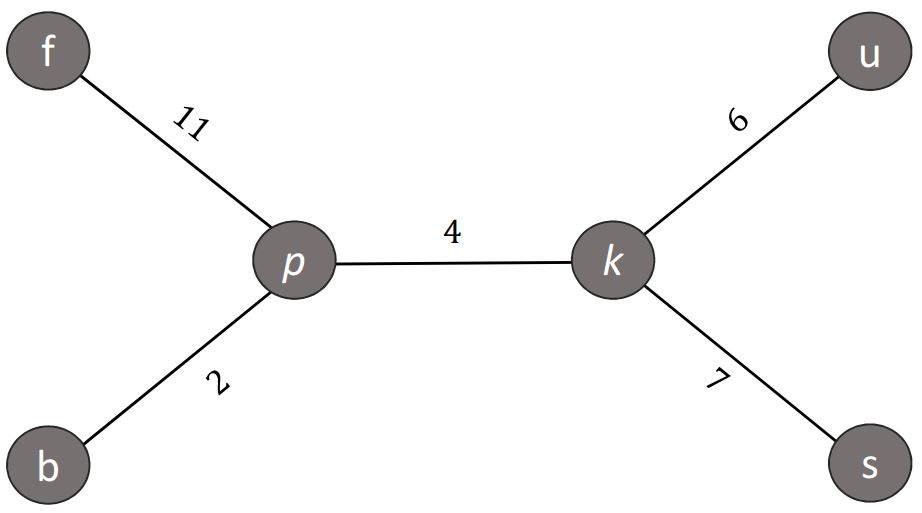
\includegraphics[height=13cm, width=11cm, keepaspectratio]{additive_tree_4.jpg}
 	\caption{Albero $T$ ottenuto da $D$.}
  	\label{fig:additivePhylogeny_4}
\end{figure}
\newline
$d_{bp}=1$ è il peso dell'arto di $b$ che è già stato calcolato in precedenza; $d_{fp}=D^{spoglia_{b}}_{f,b}=11$ è ottenuto sottraendo $limbweight(b)=2$ a $D_{f,b}=13$; $d_{pk}=4$ è dato dalla sottrazione tra $d_{fk}$ (figura 15) e $d_{fp}$ (figura 17), quindi $d_{fk}-d_{fp}=15-11=4$.
Poiché è stato costruito l'albero nella sua interezza, l'algoritmo è terminato.

\newpage
\subsection{Complessità temporale}
Di seguito viene riportato l'algoritmo scritto in pseudocodice. I parametri sono D ed n, che sono rispettivamente la matrice delle distanze adattiva di dimensione $n \times n$ e la foglia $n$.

\begin{framed}\noindent
  \textbf{AlberoAdditivo($D$, $n$)}\\
  \textbf{se} $n=2$\\
  \indent \textbf{Restituisci} l'albero costituito da un arco che collega le due foglie\\
  pesoArto $\leftarrow$ \textbf{limbweight}(n)\\
  \textbf{per} $J \leftarrow 1$ \textbf{fino a} $n-1$\\
  \indent $D_{jn} \leftarrow D_{jn} - pesoArto$\\
  \indent $D_{nj} \leftarrow D_{jn}$\\
  ($i$,$n$,$k$) $\leftarrow$ tre foglie tale che $D_{ik}=D_{in}+D_{nk}$\\
  $x \leftarrow D_{in}$\\
  \textbf{rimuovi} la riga e la colonna $n$ dalla matrice D \\
  $T \leftarrow $\textbf{AlberoAdditivo($D$, $n-1$)}\\
  $v \leftarrow $ il genitore di $n$ che è distante $x$ rispetto ad $i$ in $T$\\
  %\footnote{In altre parole è il nodo interno che viene inserito prima di poter 	  mettere la foglia (nella figura 17 sono $k$ e $p$.)} \\
  \textbf{aggiungi} la foglia $n$ a $T$ creando un arto che va tra $v$ ed $n$ il cui peso è \textit{pesoArto}
\end{framed}